\documentclass[tikz,border=10pt]{standalone}

%\documentclass{article}
\usepackage[utf8]{inputenc}
\usepackage{tikz}
\usetikzlibrary{arrows}
\usepackage{ amsmath, amssymb }
\definecolor{mio}{RGB}{0, 56, 64}
\definecolor{mio1}{RGB}{0, 90, 91}

\begin{document}


    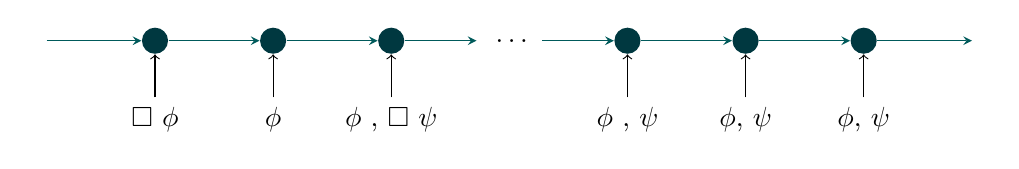
\begin{tikzpicture}[
squarednode/.style={circle, minimum size=.05mm, fill=mio},
]
%Nodes
\node[squarednode]      (Mi)    at (0,0) {};
\node[squarednode]      (Mi+1)  at (1.5,0) {};
\node[squarednode]      (Mi+2)  at (3,0) {};
\node      (Mi+3)  at (4.5,0) {\dotso};
\node[squarednode]      (Mi+4)  at (6,0) {};
\node[squarednode]      (Mi+5)  at (7.5,0) {};
\node[squarednode]      (Mi+6)  at (9,0) {};

\node (a) at  (0, -1) {$ \square \  \phi $};
\node (b) at  (1.5, -1) {$ \phi $};
\node (c) at  (3, -1) {$ \phi $ , $\square \ \psi$};
\node (g) at  (6, -1) {$ \phi $ , $\psi$};
\node (h) at  (7.5, -1) {$ \phi $, $\psi$};
\node (i) at  (9, -1) {$ \phi $, $\psi$};

\node (d) at  (-1.5, 0) {};
\node (e) at  (10.5, 0) {};

\draw[->,>=stealth, mio1] (d.east) -- (Mi.west);
\draw[->,>=stealth,mio1] (Mi.east) -- (Mi+1.west);
\draw[->,>=stealth,mio1] (Mi+1.east) -- (Mi+2.west);
\draw[->,>=stealth,mio1] (Mi+2.east) -- (Mi+3.west);
\draw[->,>=stealth,mio1] (Mi+3.east) -- (Mi+4.west);
\draw[->,>=stealth,mio1] (Mi+4.east) -- (Mi+5);
\draw[->,>=stealth,mio1] (Mi+5.east) -- (Mi+6);
\draw[->,>=stealth,mio1] (Mi+6.east) -- (e);

\draw[->] (a) -- (Mi);
\draw[->] (b) -- (Mi+1);
\draw[->] (c) -- (Mi+2);
\draw[->] (g) -- (Mi+4);
\draw[->] (h) -- (Mi+5);
\draw[->] (i) -- (Mi+6);

\end{tikzpicture}



\end{document}
